\chapter{Data} 
\label{2.Data}
\lhead{\emph{Data}}

% https://www.datacamp.com/community/tutorials/matplotlib-3d-volumetric-data


% Todo empieza con MICCAI2008
% Explota con MICCAI2016

% TODO: Improve
The two main datasets for MS lesion segmentation are those for MICCAI 2008 and MICCAI 2016 challenges. In this project we'll work over MICCAI 2016 dataset.

\section{MICCAI 2016 dataset}

% TODO: Modalities/Channels!!
MICCAI 2016 dataset consists on 15 MRIs together with a lession mask generated by consensus among various doctors. These are generated with three different scanners, each one with a certain data shape. We verified that all the MRIs are present with the same orientation, what will be meaningfull when slicing the 3-D MRIs for the 2-D models. The dataset contains also preprocessed data in which the skull has been removed from the MRIs, for simplicity, we'll be using these for all the models.

We split randomly the data in a train and a validation set with size 12 and 3 MRIs respectively. We don't keep a test set because given the fact that the size of this would be reduced to only one or two MRIs at most and the inhomogeneity in the different lesions shape, size, quantity and distribution, the evaluation over the test set would lead to a unreliable measurement. This is something certain after seeing the big differences in the metrics over different validation MRIs. Therefore we encourage to everyone who wants to use this models in practice to previously evaluate them over his own data.

We present in the next page some slices of MRIs used as benchmarks for error detection and visual analysis of the models from both the train and validation datasets.

\newpage
Becnhmark training images:
\begin{figure*}[!htb]
    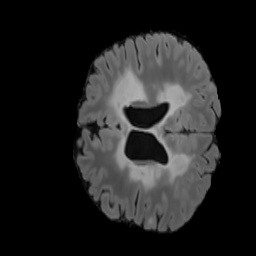
\includegraphics[width=.32\textwidth]{images/tr_images/tr175_input.jpg}\hfill
    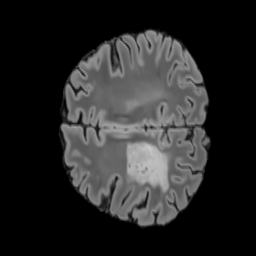
\includegraphics[width=.32\textwidth]{images/tr_images/tr943_input.jpg}\hfill
    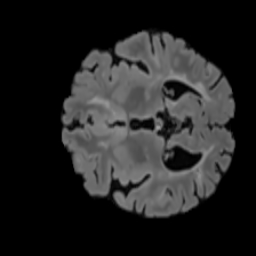
\includegraphics[width=.32\textwidth]{images/tr_images/tr1426_input.jpg}
    %\caption{Image A.}
    %\caption{Image B.}
    %\caption{Image C.}
    \subfigure[tr175]{
\includegraphics[width=.32\textwidth]{images/tr_images/tr175_mask.jpg}\label{fig:tr175}}\hfill
    \subfigure[tr943]{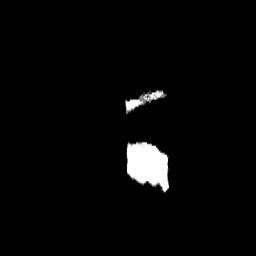
\includegraphics[width=.32\textwidth]{images/tr_images/tr943_mask.jpg}\label{fig:tr943}}\hfill
    \subfigure[tr1426]{
\includegraphics[width=.32\textwidth]{images/tr_images/tr1426_mask.jpg}\label{fig:tr1426}}
    %\caption{Image A.}
    %\caption{Image B.}
    %\caption{Image C.}
\end{figure*}

Benchmark validation images: 
\begin{figure*}[!htb]
    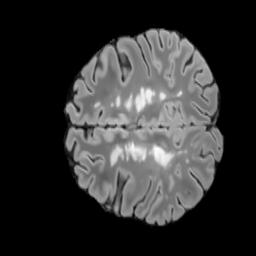
\includegraphics[width=.32\textwidth]{images/ts_images/ts175_input.jpg}\hfill
    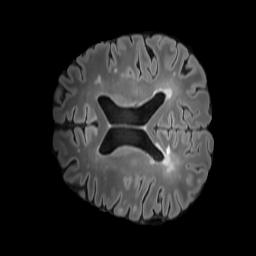
\includegraphics[width=.32\textwidth]{images/ts_images/ts431_input.jpg}\hfill
    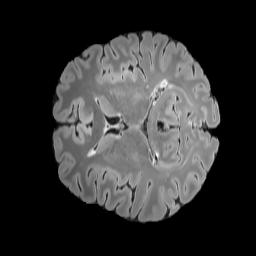
\includegraphics[width=.32\textwidth]{images/ts_images/ts687_input.jpg}
    %\caption{Image A.}
    %\caption{Image B.}
    %\caption{Image C.}
    \subfigure[ts175]{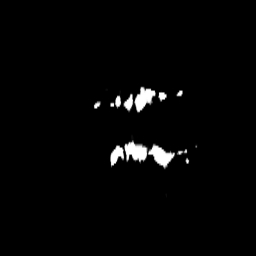
\includegraphics[width=.32\textwidth]{images/ts_images/ts175_mask.jpg}\label{fig:ts175}}\hfill
    \subfigure[ts431]{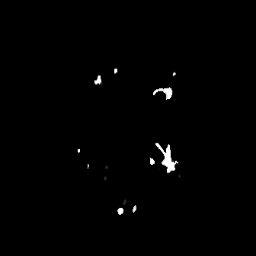
\includegraphics[width=.32\textwidth]{images/ts_images/ts431_mask.jpg}\label{fig:ts431}}\hfill
    \subfigure[ts687]{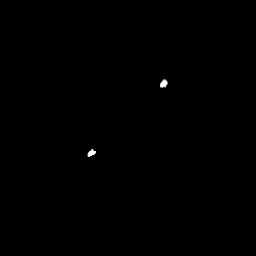
\includegraphics[width=.32\textwidth]{images/ts_images/ts687_mask.jpg}\label{fig:ts687}}
    %\caption{Image A.}
    %\caption{Image B.}
    %\caption{Image C.}
\end{figure*}

\newpage
\section{Evaluation metrics}

%%%%%%%%%%%%%%%%%% Listing configuration %%%%%%%%%%%%%%%%%
\definecolor{gray97}{gray}{.97}
\definecolor{gray75}{gray}{.75}
\definecolor{gray45}{gray}{.45}

\lstset{ frame=Ltb,
framerule=0pt,
aboveskip=0.5cm,
framextopmargin=3pt,
framexbottommargin=3pt,
framexleftmargin=0.4cm,
framesep=0pt,
rulesep=.4pt,
backgroundcolor=\color{gray97},
rulesepcolor=\color{black},
%
stringstyle=\ttfamily,
showstringspaces = false,
basicstyle=\fontsize{9.5}{10}\selectfont\ttfamily,
commentstyle=\color{gray45},
keywordstyle=\bfseries,
%
numbers=left,
numbersep=15pt,
numberstyle=\tiny,
numberfirstline = false,
breaklines=true,
}

% minimizar fragmentado de listados
\lstnewenvironment{listing}[1][]
{\lstset{#1}\pagebreak[0]}{\pagebreak[0]}

\lstdefinestyle{consola}
{basicstyle=\scriptsize\bf\ttfamily,
backgroundcolor=\color{gray75},
}

\lstdefinestyle{C}
{language=Python,
}
%%%%%%%%%%%%%%%%%%%%%%%%%%%%%%%%%%%%%%%%%%%%%%%%%%%%%%%%%%

During the training processes we have used \textit{binary cross entropy} as loss function. For evaluation we have used the \textit{Dice score}, a classical metric for image segmentation, much more representative than others used in classification tasks as \textit{Mean Squared Error} or \textit{Binary accuracy}. \textit{Dice score} is implemented in several similar but not fully equivalent ways and it's not a built-in metric in keras-tensorflow so we had to create our custom implementations for both the tensorflow and PyEDDL models. This way we also ensure they are strictly equivalent.

\begin{equation*}
Dice(Pred, Mask) = 2*\frac{|Pred \cap Mask |}{|Pred| + |Mask|} 
\end{equation*}
\vspace{10pt}

\begin{lstlisting}[language=Python, caption=Keras backend Dice implementation]
import keras.backend as K

def dice(y_true, y_pred, smooth=1):
    intersection = K.sum(y_true * y_pred, axis=[1,2,3])
    union = K.sum(y_true, axis=[1,2,3]) + K.sum(y_pred, axis=[1,2,3])
    dice = K.mean((2. * intersection + smooth)/(union + smooth), axis=0)
    return dice
\end{lstlisting}

\begin{lstlisting}[language=Python, caption=PyEDDL Dice implementation]
from pyeddl._core  import Metric

class Dice(Metric):
    def __init__(self, threshold=0.5):
        Metric.__init__(self, "py_dice")
        self.threshold = threshold

    def value(self, msk, out, smooth=1):   
        out_np = out.getdata() >= self.threshold
        msk_np = msk.getdata().astype(np.bool)
        intersection = np.logical_and(msk_np, out_np)
        
        dice = 0
        for i in range(msk_np.shape[0]):
            union_i = np.sum(msk_np[i]) + np.sum(out_np[i])
            dice += (2*np.sum(intersection[i])+smooth) / (union_i+smooth)

        return dice

\end{lstlisting}